\documentclass[../DS07.tex]{subfiles}
\graphicspath{{./figures/}}

% \subimport{/home/nora/Documents/Enseignement/Prepa/bpep/exercices/DS/pendule_et_effets_non_lineaires/}{sujet.tex}

\begin{document}
\exercice[23]{Balançoire\ifcorrige{~\small\textit{(D'après CCP 2013)}}}

\renewcommand{\version}{frottements}

\enonce{
	Un enfant faisant de la balançoire (figure \ref{fig:balancoire}) est modélisé
	par une masse ponctuelle $m$ située en $M$ et suspendue en $O$ par une corde
	de masse négligeable et de longueur $\ell$. Le champ de pensanteur $\gf$, de
	norme $g$, est supposé uniforme. L'angle que fait la corde de suspension avec
	la verticale est noté $\th$. Les vecteurs unitaires $\ur$,
	$\ut$ et $\uz=\ur\wedge \ut$ tels que
	définis sur la figure \ref{fig:balancoire_schema} définissent un trièdre
	orthonomé direct lié à la balançoire.
	\noindent
	\begin{minipage}[c]{.46\linewidth}
		\begin{center}
			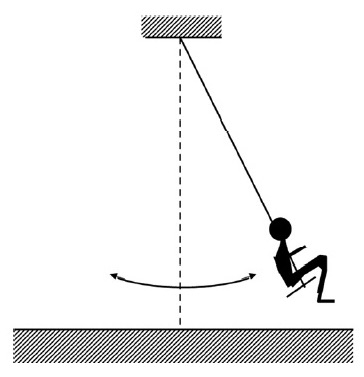
\includegraphics[height=5cm]{balancoire}
			\captionof{figure}{Enfant assis sur sa balançoire.}
			\label{fig:balancoire}
		\end{center}
	\end{minipage}
	\hfill
	\begin{minipage}[c]{.46\linewidth}
		\vspace{0pt}
		\begin{center}
			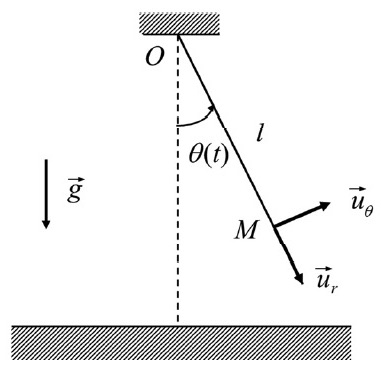
\includegraphics[height=5cm]{balancoire_schema}
			\captionof{figure}{Schématisation de la balançoire.}
			\label{fig:balancoire_schema}
		\end{center}
	\end{minipage}
}

\enonce{
	Dans toute la suite du problème, les mouvements de la balançoire et de
	l'enfant seront étudiés dans le plan de la figure \ref{fig:balancoire_schema}.
	% De plus, les parties \ref{part:nl} et \ref{part:frottement} sont
	% indépendantes.
	\begin{tcb}*(exem)<itc>"odgr"{Aide au calcul}
		\[
			(a+b)^3 = a^3 + 3a^2 b + 3ab^2 + b^3
			\qquad ; \qquad
			\cos^3x=\dfrac{3\cos x+\cos (3x)}{4}
		\]
	\end{tcb}
}

\subsection{Mise en équation}

\enonce{%
	Sauf mention contraire dans la suite de l'énoncé, %tout frottement de la tige sur son axe de rotation et
	tout frottement dû à la résistance de l'air est négligé.
}

\QR{\label{q:mee}
	Etablir l'équation différentielle nommée~(E) du mouvement vérifiée par
	$\th(t)$ en utilisant 3 méthodes~:
	\begin{itemize}
		\item en appliquant le principe fondamental de la dynamique
		\item en appliquant un théorème énergétique
		\item en appliquant le théorème du moment cinétique
	\end{itemize}
}{%
	On étudie l'enfant (assimilé à un point matériel) dans le référentiel lié au
	sol et supposé galiléen dans la base polaire $(O, \ur, \ut)$.
	On effectue le bilan des actions extérieures suivant~:
	\begin{itemize}
		\item Le poids $\Pf = mg \cos(\th)\ur - mg \sin(\th) \ut$ avec de plus
		      $\Ec_{pp} = - mgl \cos(\th) $ puis $\Mcf_O(\Pf) = l \ur \wedge \Pf = -lmg \sin(\th)
			      \ez $.
		\item La tension du fil $\Tf = -T \ur$ avec $T >0$ tant que le fil
		      est tendu. Cette force ne travaille pas (puissance nulle car $\Tf \cdot
			      \vf = 0$) et son moment par rapport à $O$ est aussi nul (support de
		      force passant par $O$).
	\end{itemize}
	De plus, une étude cinématique du problème indique $\vf = l \tp
		\ut$ puis $\af = l \tpp \ut - l (\tp)^2 \ur$ et finalement $\Lcf _O(M) = \OM
		\wedge m \vf = ml^2 \tp \ez$.
	\smallbreak
	On peut donc appliquer les trois méthodes proposées par l'énoncé~:
	\begin{itemize}
		\item On applique le principe fondamental de la dynamique à l'enfant dans le
		      référentiel galiléen en projection selon $\ut$
		      \[
			      ml \tpp =  mg \sin(\th) \Rightarrow \boxed{ \dv[2]{\th}{t} + \frac{g}{l}\sin(\th) = 0}
		      \]
		\item On applique le théorème de la puissance mécanique à l'enfant dans le référentiel galiléen
		      \[
			      \dv{\Ec_m}{t} =
			      P_{nc} = 0
			      \Rightarrow
			      ml^2 \tp\tpp + mgl \tp \sin(\th) = 0
			      \Rightarrow
			      \boxed{ \dv[2]{\th}{t} + \frac{g}{l}\sin(\th) = 0}
		      \]

		\item Enfin, on applique le théorème du moment cinétique (TMC) à l'enfant
		      par rapport au point $O$  dans le référentiel galiléen et en projection
		      selon $\ez$
		      \begin{gather*}
			      \dv{\Lcf _0(M)}{t} \cdot \ez =
			      \Mc _0(\Pf) \cdot \ez
			      \Rightarrow
			      \boxed{ \dv[2]{\th}{t} + \frac{g}{l}\sin(\th) = 0}
			      \tag{E}
			      \label{eq:TMC}
		      \end{gather*}
	\end{itemize}
	On obtient bien dans les trois cas le même résultat.
}

\QR{%
	À quelle condition l'enfant assis sur la balançoire sera-t-il assimilé à un
	oscillateur harmonique~? Donner l'expression de la pulsation propre $\w_0$
	correspondante.
}{%
	Lorsque $\abs{\th} \ll 1$ (en radian), on a $\sin(\th) \approx  \th$ et
	on obtient l'équation de l'oscillateur harmonique. On en déduit par
	identification que $\boxed{\w_0 = \sqrt{g/l}}$.
}

\QR{%
	Application numérique~: L'enfant part d'un angle $\th_0=30$° sans vitesse
	initiale. On donne les valeurs numériques suivantes~: $l=\SI{2,5}{m}$ ,
	$g=\SI{10}{m.s^{-2}}$ et $m=\SI{20}{kg}$. Calculer la période $T_0$ de
	l'oscillateur harmonique, ainsi que la vitesse maximale $v_{\max}$ de l'enfant.
}{%
	On a $T_0 = 2\pi / \w_0 \approx \SI{3,1}{s} $. De plus, on obtient
	$\th(t) = A \cos(\w_0 t + \phi)$ or à $t=0$, la vitesse initiale est
	nulle et on en déduit que $-A \sin(\phi)=0$ soit $\phi=0$ qui convient. La
	deuxième CI sur l'angle initial donne donc au final $\th(t) = \th_0
		\cos(\w_0 t)$.
	\smallbreak
	On obtient alors l'expression de la vitesse en dérivant soit $v(t) = l
		\tp = -\th_0 l \w_0 \sin(\w_0 t)$ et donc la vitesse
	maximale à pour expression $v_{\max} = l \w_0 \th_0$.

	\textbf{Pour aller plus loin}~:
	\smallbreak
	On peut retrouver ce résultat plus rapidement à l'aide de l'étude
	energétique. On a $\Ec_c$ max lorsque $\Ec_p$ passe par son miminum pour un
	système conservatif. Cela arrive pour $\th = 0$ et on en déduit
	$\Ec_{c,\max} = \Ec_m - \Ec_p(0)$ soit au final
	\[
		\Ec_{c,\max} =
		\frac{1}{2}m v_{\max}^2 =
		mgl(1-\cos(\th_0)) \approx
		mgl \frac{\th_0^2}{2}
		\Rightarrow
		\sqrt{gl} \th_0
	\]
	à l'aide d'un développement limité à l'ordre 2. Ce résultat est bien
	identique à celui obtenu précédemment.
}

\subsection{Etude d'une solution non harmonique}
\label{part:nl}
\enonce{
	On souhaite obtenir une modélisation plus précise des oscillations en prenant
	en compte une partie des effets non linéaires. On considère toujours dans
	cette partie que l'enfant part d'un angle $0<\th_0 \ll 1$ et sans vitesse
	initiale.
}

\QR{%
	En posant $\sin \th = \th - \th^3/6$, que devient l'équation
	différentielle~(E) du mouvement vérifiée par $\th(t)$~? Cette
	équation, appelée (E') est-elle encore linéaire~?
}{%
	L'équation~\eqref{eq:TMC} devient simplement
	\begin{equation}
		\dv[2]{\th}{t} + \w_0^2\th -\w_0^2 \th^3/6 = 0
		\label{eq:TMCDL}
		\tag{E'}
	\end{equation}
	On observe alors que cette équation n'est plus linéaire (présence de
	l'inconnue à la puissance trois).
}

\begin{blocQR}
	\item
	\enonce{%
		On cherche, pour cette équation différentielle approchée une solution
		elle-même approchée de la forme
		\[
			\th(t) =
			\th_0\cos(\w t) + \ep \th_0\cos(3\w t)
			\qMath{où}
			\ep\ll 1
			\qet
			\th_0 \ll 1
		\]
	}
	\QR{\label{q:approx_tri}
	En utilisant les approximation proposée par l'énoncé, montrer que le terme
	$\th^3/6$ peut se simplifier en
	\[
		\frac{\th^3}{6} = \frac{\th_0^3}{24} \pa{3 \cos(\w t) + \cos(3\w t)}
	\]
	}{%
	On a ici
	\[
		\frac{\th^3}{6} =
		\frac{\th_0^3}{6}
		\pa{ \cos^3(\w t) +
		\underbracket[1pt]{3 \ep \cos^2(\w t)\cos(3\w t) +
			3 \ep^2 \cos(\w t)\cos^2(3\w t) +
			\ep^3 \cos^3(3\w t)}_
		{\text{négligeable}}}
	\]
	Parmis ces quatre termes, on ne conserve que le premier car les autres sont
	négligeables ($\ep \ll 1$). On utilise alors les résultats
	trigonométriques fournis par l'énoncé pour obtenir l'expression demandée
	\[
		\frac{\th^3}{6} \approx
		\frac{\th_0^3}{6} \cos^3(\w t) =
		\frac{\th_0^3}{6}
		\pa{\frac{3}{4} \cos(\w t) +
			\frac{1}{4} \cos(3\w t)} =
		\frac{\th_0^3}{24} \pa{3 \cos(\w t) + \cos(3\w t)}
	\]
	d'où le résultat.
	}

	\QR{\label{q:lemme}
		Démontrer le résultat suivant
		\[
			\forall t~:
			A \cos(\w t) =
			B \cos(3 \w t)
			\quad \Rightarrow \quad
			A=B=0
		\]
	}{%
		On se place dans un premier temps à $t=0$, on en déduit $A=B$. On considère
		maintenant l'instant $t_i$ tel que $\w t_i = \pi/3$. On obtient alors $A
			\cos(\pi/3) = B\cos(\pi) \Rightarrow  A/2 = -B = -A \Rightarrow A=B=0$ d'où
		le résultat.

		\corrigeBonus{
			On peut aussi obtenir ce résultat (une fois l'égalité entre $A$ et $B$
			établie) en dérivant la relation
			\[
				-A \w \sin(\w t) = -3A \w(\sin(3 \w t))
			\]
			et en se plaçant à l'instant $t_j$ tel que $\w t_j=\pi/2$ ce qui donne
			après simplification $A = -3A \Rightarrow A=B=0$.}
	}

	\QR{%
		Exprimer en fonction de $\w_0$ et $\th_0$ la pulsation fondamentale
		$\w$ ainsi que le terme $\ep$ en injectant l'expression proposée
		pour $\th(t)$ dans l'équation~(E') et en utilisant
		l'approximation établie à la question \ref{q:approx_tri}.
		\smallbreak
		On montera en particulier que
		$\w=\w_0\sqrt{1-\frac{1}{8}\th_0^2}$ et
		$\ep=\dfrac{\th_0^2}{-192+27\th_0^2}$.
	}{%
		On injecte la solution proposée dans l'équation~\eqref{eq:TMCDL} et on regroupe
		les termes en $\cos(\w t)$ et $\cos(3 \w t)$.
		\[
			\pa{
				-\th_0 \w^2 +
				\th_0 \w_0^2 -
				\frac{\w_0^2}{8} \th_0^3}
			\cos(\w t) =
			\pa{
				\ep \th_0 9 \w^2 -
				\ep \th_0 \w_0^2 +
				\frac{\w_0^2}{24}\th_0^3}
			\cos(3\w t)
		\]
		On utilise alors le résultat établi à la question \ref{q:lemme} pour obtenir
		un système de deux équations à deux inconnues ($\w$ et $\ep$)
		que l'on simplifie sachant que $\th_0 \neq 0$
		\begin{align*}
			- \w^2 + \w_0^2 - \frac{\w_0^2}{8} \th_0^2 & =
			0
			\label{eq:a}
			\tag{a}
			\\
			\ep 9 \w^2 - \ep \w_0^2 +
			\frac{\w_0^2}{24}\th_0^2                   & =
			0
			\label{eq:b}
			\tag{b}
		\end{align*}
		De l'équation~\eqref{eq:a}, on obtient $\boxed{\w =
				\w_0\sqrt{1-\frac{\th_0^2}{8}}}$ soit le résultat attendu. On peut
		alors reconsidérer l'équation~\eqref{eq:b} en substituant $\w^2$ par son
		expression
		\[
			\ep 9 \w_0^2
			\pa{
				1-
				\frac{\th_0^2}{8}} -
			\ep \w_0^2 +
			\frac{\w_0^2}{24}\th_0^2 =
			0
			\Rightarrow
			\ep
			\pa{8- \frac{9}{8}\th_0^2} =
			- \frac{\th_0^2}{24}
			\Rightarrow
			\boxed{\ep = \frac{\th_0^2}{27\th_0^2-192}}
		\]
		d'où le résultat.
	}

\end{blocQR}

\QR{%
	Par rapport au mouvement harmonique, le signal $\th (t)$ a-t-il une plus
	grande ou une plus petite période~?
}{%
	On observe dans un premier temps que la période de $\th(t)$ a pour
	expression $T=2\pi /\w$. En effet, ce terme est aussi une période (mais
	non la plus petite) pour l'expression $\cos(3\w t)$.
	\smallbreak
	On a donc
	\[
		T = \frac{2\pi}{\w} = \underbracket[1pt]{\frac{2\pi}{\w_0}}_{=T_0} \frac{1}{\sqrt{1-\frac{\th_0^2}{8}}}
	\]
	et on en déduit alors que $\boxed{T > T_0}$. La période des oscillations
	augmente alors légèrement avec l'angle $\th_0$.
	\smallbreak
	On retrouve bien au passage que $T \to T_0$ lorsque $\th_0 \to 0$ ce qui
	est bien le résultat attendu.
}

\QR{%
	Quelle est la pulsation du premier harmonique après le fondamental~?
}{%
	L'expression de $\th(t)$ correspond déjà au développement en série de
	Fourier d'un signal. On observe alors directement que le premier harmonique à
	pour pulsation $\boxed{\w_3=3 \w}$.
}

% \subsection{Prise en compte des frottements fluides}
% \label{part:frottement}
%
% \enonce{
% 	On prend maintenant en considération les forces de frottement de l'air et on
% 	néglige tout effet non linéaire. Le moment de ces forces par rapport à $O$ est
% 	égal à $-C\dv{\th}{t} \ez$ où $C$ est une constante positive.
% }
%
% \QR{
% Quelle est la dimension de la constante $C$~?
% }{%
% On a
% \[
% 	{\rm M.L^2.T^{-2}} =
% 	\dim{ \Mc_0(\Ff)} =
% 	\dim(-C \tp)
% 	\Rightarrow
% 	\dim{C} = {\rm M.L^2.T^{-1}}
% \]
% }
%
% \QR{
% 	En reprenant les éléments apportés lors de la réponse à la question
% 	\label{q:mee}, établir l'équation différentielle linéaire nommée (E'') à
% 	laquelle doit maintenant obéir $\th(t)$.
% }{%
% 	Il convient d'ajouter une nouvelle action dans le bilan des actions exercées
% 	sur la masse. L'application du TMC à l'enfant par rapport au point $O$ et en
% 	projection selon $\ez$ donne
% 	\begin{gather*}
% 		\dv{\Lcf _0(M)}{t}\ez =
% 		\Mcf_0(\Pf)\ez - C \dv{\th}{t}
% 		\Rightarrow
% 		\boxed{
% 			\dv[2]{\th}{t} +
% 			\frac{C}{ml^2}\dv{\th}{t} +
% 			\w_0^2 \th =
% 			0}
% 		\label{eq:TMCfrott}
% 		\tag{E''}
% 	\end{gather*}
% }
%
% \QR{
% 	À quelle inégalité doit satisfaire $C$ pour que le mouvement de l'enfant
% 	puisse être considéré comme un mouvement oscillatoire dont l'amplitude décroît
% 	avec le temps (régime pseudo-périodique)~?
% }{%
% 	On obtient un régime pseudo-périodique lorsque le discriminant de l'équation
% 	caractéristique associée est négatif soit ici lorsque
% 	\[
% 		\frac{C}{ml^2}^2 - 4 \w_0^2 <0 \Rightarrow \boxed{C < 2 \w_0 ml^2}
% 	\]
% 	On observe au passage que ce résultat est compatible avec la dimension de $C$
% 	obtenue précédemment.
% }
%
% \QR{
% 	Montrer, toujours dans le cas du régime pseudo-périodique, que la solution de
% 	l'équation~(E'') s'exprime sous la forme
% 	\[
% 		\th(t) = A e^{-\frac{C}{2ml^2} t}\cos(\w t + \phi)
% 	\]
% 	avec $\w = \w_0\sqrt{1 - \frac{C}{4ml^2\w_0^2}}$ et sans chercher
% 	à établir les expression de $A$ et $\phi$.
% }{%
% 	L'équation caractéristique à pour solutions
% 	\[
% 		r_{\pm} = -\frac{C}{2ml^2} \pm \jj \frac{ 4 \w_0^2 - \frac{C}{ml^2}^2}{2}
% 	\]
% 	On en déduit alors que la solution générale de l'équation~\eqref{eq:TMCfrott}
% 	s'exprime selon
% 	\[
% 		\boxed{\th(t) = A e^{-\frac{C}{2ml^2} t}\cos(\w_0\sqrt{1 - \frac{C}{4ml^2\w_0^2}} t + \phi)}
% 	\]
% 	avec $A$ et $\phi$, deux constantes à exprimer à l'aide des conditions
% 	initiales (non demandé ici car ces conditions initiales ne sont pas
% 	fournies).
% }
%
% \QR{
% 	L'enfant part d'un angle $\th_0 = 15$° sans vitesse initiale. On observe
% 	que l'amplitude du mouvement est réduite de moitié après 20 oscillations.
% 	Comment se simplifie alors l'expression de $\w$~?
% 	\smallbreak
% 	Application numérique~: calculer la valeur de la constante $C$.
% }{%
% 	On observe donc au moins 20 oscillations ce qui implique que le facteur de
% 	qualité est élevé et donc que $\w \approx \w_0$. On reprend alors le
% 	résultat établi à la question suivante avec $T = 2\pi/\w_0$
% 	\[
% 		A e^{-\frac{C}{2ml^2} 20T} = A/2
% 		\Rightarrow
% 		\frac{C}{2ml^2} 20T = \ln(2)
% 		\Rightarrow
% 		\boxed{
% 			C = ml^2 \frac{ \ln(2)}{20\pi} \sqrt{\frac{g}{l}} \approx
% 			\SI{5,5}{kg . m^2 . s^{-1}}
% 		}
% 	\]
% }

\end{document}
